\documentclass[14pt, a4paper]{extarticle}
\usepackage{GOST}
\usepackage{array}
\usepackage{verbatim}
\usepackage[detect-all]{siunitx}
\usepackage{amsmath}
\usepackage{amssymb}
\usepackage[utf8]{inputenc}
\usepackage{hyperref}

\usepackage{ifthen}


\usepackage{tempora}



\makeatletter
\renewcommand\@biblabel[1]{#1.}
\makeatother

% Для листинга кода:
\usepackage{listings}
\lstset{ %
	language=c++,                 % выбор языка для подсветки (здесь это С)
	basicstyle=\small\sffamily, % размер и начертание шрифта для подсветки кода
	numbers=left,               % где поставить нумерацию строк (слева\справа)
	numberstyle=\tiny,           % размер шрифта для номеров строк
	stepnumber=1,                   % размер шага между двумя номерами строк
	numbersep=5pt,                % как далеко отстоят номера строк от подсвечиваемого кода
	showspaces=false,            % показывать или нет пробелы специальными отступами
	showstringspaces=false,      % показывать или нет пробелы в строках
	showtabs=false,             % показывать или нет табуляцию в строках
	frame=single,              % рисовать рамку вокруг кода
	tabsize=2,                 % размер табуляции по умолчанию равен 2 пробелам
	captionpos=t,              % позиция заголовка вверху [t] или внизу [b] 
	breaklines=true,           % автоматически переносить строки (да\нет)
	breakatwhitespace=false, % переносить строки только если есть пробел
	escapeinside={\#*}{*)}   % если нужно добавить комментарии в коде
}


%для графиков
\usepackage{pgfplots}
\usepackage{filecontents}
\usetikzlibrary{datavisualization}
\usetikzlibrary{datavisualization.formats.functions}

\begin{document}
	
	\begin{table}[ht]
		\centering
		\begin{tabular}{|c|p{400pt}|} 
			\hline
			\begin{tabular}[c]{@{}c@{}} 
\includegraphics[scale=1]{baum.jpg} \\\end{tabular} &
			\footnotesize\begin{tabular}[c]{@{}c@{}}\textbf{Министерство~науки~и~высшего~образования~Российской~Федерации}\\\textbf{Федеральное~государственное~бюджетное~образовательное~учреждение}\\\textbf{~высшего~образования}\\\textbf{«Московский~государственный~технический~университет}\\\textbf{имени~Н.Э.~Баумана}\\\textbf{(национальный~исследовательский~университет)»}\\\textbf{(МГТУ~им.~Н.Э.~Баумана)}\\\end{tabular}  \\
			\hline
		\end{tabular}
	\end{table}
	\noindent\rule{\textwidth}{4pt}
	\noindent\rule[14pt]{\textwidth}{1pt}
	\hfill 
	\noindent
	\makebox{ФАКУЛЬТЕТ~}%
	\makebox[\textwidth][l]{\underline{~«Информатика и системы управления»~~~~~~~~~~~~~~~~~~~~~~~~~~~~~~~~~}}%
	\\
	\noindent
	\makebox{КАФЕДРА~}%
	\makebox[\textwidth][l]{\underline{~«Программное обеспечение ЭВМ и информационные технологии»~}}%
	\\
	
	\begin{center}
		\vspace{1.5cm}
		{\bf\huge Отчёт\par}
		{\bf\Large по лабораторной работе № 5\par}
		\vspace{0.7cm}
	\end{center}
	
	
	\noindent
	\makebox{\large{\bf Название:}~~~}
	\makebox[\textwidth][l]{\large\underline{Многопоточная реализация конвейера~~~~~~~~~~~~~}}\\
	
	\noindent
	\makebox{\large{\bf Дисциплина:}~~~}
	\makebox[\textwidth][l]{\large\underline{~Анализ алгоритмов~~~~~~~~~~~~~~~~~~~~~~~~~~}}\\
	
	\vspace{1.5cm}
	\noindent
	\begin{tabular}{l c c c c c}
		Студент      & ~ИУ7-55Б~               & \hspace{2.5cm} & \hspace{2cm}                 & &  Д.В. 
		Сусликов \\\cline{2-2}\cline{4-4} \cline{6-6} 
		\hspace{3cm} & {\footnotesize(Группа)} &                & {\footnotesize(Подпись, дата)} & & {\footnotesize(И.О. Фамилия)}
	\end{tabular}
	
	\noindent
	\begin{tabular}{l c c c c}
		Преподователь & \hspace{5cm}   & \hspace{2cm}                 & & ~~~~~~Л.Л. Волкова~~~~~~\\\cline{3-3} \cline{5-5} 
		\hspace{3cm}  &                & {\footnotesize(Подпись, дата)} & & {\footnotesize(И.О. Фамилия)}
	\end{tabular}
	
	\vspace{0.6cm}
	\begin{center}	
		\vfill
		\large \textit {Москва, 2020}
	\end{center}
	
	\thispagestyle {empty}
	\pagebreak
	
	% СОДЕРЖАНИЕ 
	\clearpage
	\tableofcontents
	
	
	% ВВЕДЕНИЕ
	\clearpage
	\section*{Введение}
	\addcontentsline{toc}{section}{Введение}
	Цель работы: создание системы конвейерных вычислений.\par
	В ходе лабораторной работы требуется:
	\begin{enumerate}
		\item[1)] дать описание алгоритма реализации конвейерных вычислений;
		\item[2)] реализовать данный алгоритм;
		\item[3)] провести его тестирование.
	\end{enumerate}\par
	 
	\clearpage
	\section{Аналитический раздел}
	В данном разделе представлены принципы конвейерных вычислений и параллельных.
	
	\subsection{Общие сведения}
	Конвейерное производство — система поточной организации производства на основе конвейера, при которой оно разделено на простейшие короткие операции, а перемещение деталей осуществляется автоматически. Это такая организация выполнения операций над объектами, при которой весь процесс воздействия разделяется на последовательность стадий с целью повышения производительности путём одновременного независимого выполнения операций над несколькими объектами, проходящими различные стадии.
	
	Конвейером также называют средство продвижения объектов между стадиями при такой организации\hyperref[Conveyer]{[4]}.
	
	\subsection{Параллельные вычисления}
	Параллельные вычисления – способ организации компьютерных вычислений, при котором программы разрабатываются как набор взаимодействующих вычислительных процессов, работающих параллельно (одновременно). Термин охватывает совокупность вопросов параллелизма в программировании, а также создание эффективно действующих аппаратных реализаций. Теория параллельных вычислений составляет раздел прикладной теории алгоритмов\hyperref[ParInfo]{[5]}.
	
	
	\subsection*{Вывод}
	\addcontentsline{toc}{subsection}{Вывод}
	По итогу, были разобраны общая информация о конвейерном производстве и конвейерах и суть параллельных вычислений.
	
	\section{Конструкторский раздел}
	В данном разделе представлена схема алгоритмов обработки элементов линии конвейера, а также описана сама система.
	\subsection{Разработка алгоритма}
	На Рисунке 1 изображена схема алгоритмов обработки элементов линии конвейера.
	\begin{figure}[h!]
		\centering{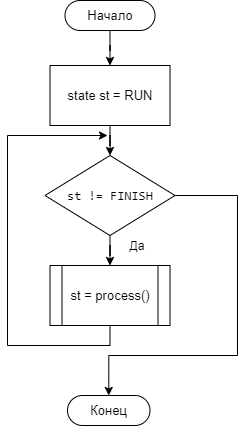
\includegraphics[scale=1]{start.png}}
		\caption{Схема алгоритма старта и процесса линии конвейера}
	\end{figure}
	\clearpage
	
	На Рисунке 2 можно увидеть схему алгоритма обработки элементов линии конвейера.
	\begin{figure}[h!]
		\centering{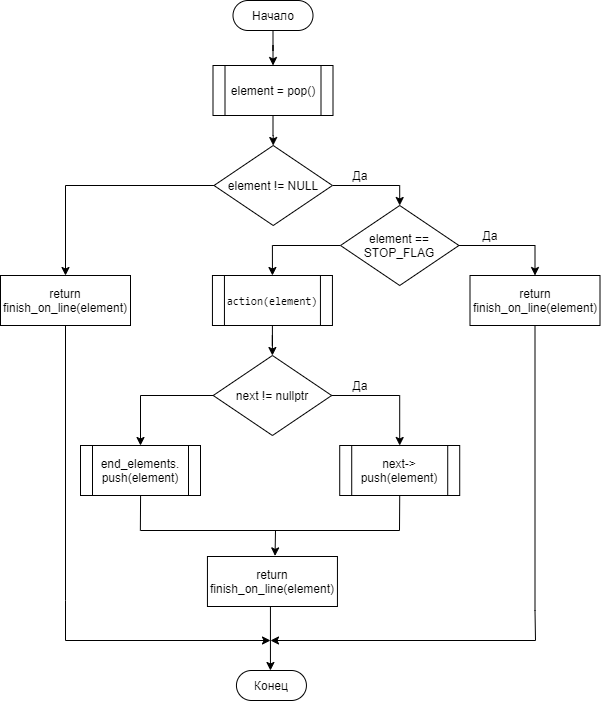
\includegraphics[scale=0.8]{process.png}}
		\caption{Схема алгоритма обработки элементов линии конвейера}
	\end{figure}
	\clearpage
	
	
	\subsection{Описание системы}
	Система состоит из 3 параллельно работающих линий. Каждая линия имеет указатель на следующую, кроме последней, которая указывает на $nullptr$. Изначально задаётся очередь элементов, последний из которых является флагом окончания очереди $STOP\_FLAG$. Каждый элемент поочередно записывается на первую линию, обрабатывается и посылается на следующую линию. Время о поступлении и выхода с линии и другая информация своевременно выводятся на экран. С последней линии элементы записываются в результирующий массив $end\_elements$ для последующего вывода.  
	
	\subsection*{Вывод}
	\addcontentsline{toc}{subsection}{Вывод}
	Таким образом, были разобраны схема алгоритмов обработки элементов линии конвейера, а также сама система.
	
	\section{Технологический раздел}
	В данном разделе даны общие требования к программе, средства реализации и реализация алгоритмов.
	
	\subsection{Общие требования}
	Требование:
	\begin{enumerate}
		\item[1)] аргументы должны последовательно проходить линии в заданном порядке;
		\item[2)] каждая линия должна работать в своем потоке;
		\item[3)] последним элементом должен быть флаг, при поступлении которого, линия должна завершить свою работу;
		\item[4)] при пустой очереди линии, она должна ожидать поступления нового элемента;
		\item[5)] в результате из последней линии должен вернуться массив аргументов, у которого порядок совпадает с начальным.
	\end{enumerate}

	\subsection{Средства реализации}
	В лабораторной работе был использован язык $C$++\hyperref[CPlusPlus]{[1]}, так как он известен, и на нём было написано множество предыдущих работ.
	
	Среда разработки - $Qt$\hyperref[Cute]{[2]}.
	
	Для замеров процессорного времени была использована функция $clock()$\hyperref[CLOCK]{[3]}.
	\newpage
		
	\subsection{Реализация алгоритмов}
	В Листинге 1 реализован алгоритм старта линии конвейера.\newline
	Листинг 1 -	Алгоритм старта линии конвейера
	\begin{lstlisting}	
		void ConveyerLine::start_line()
		{
			state st = RUN;
			while (st != FINISH)
				st = process();
		}
	\end{lstlisting}
		
	В Листинге 2 реализован алгоритм обработки аргумента линии.\newline
	Листинг 2 - Алгоритм обработки аргумента линии
	\begin{lstlisting}	
		state ConveyerLine::process()
		{
			int element = pop();
			if (element != NULL)
			{
				if (element == STOP_FLAG)
					return finish_on_line(element);
				
				action(element);
				
				if (next != nullptr)
					next->push(element);
				else
					end_elements.push(element);
			}
			else
				return STOP;
			
			return RUN;
		}
	\end{lstlisting}
	В Листинге 3 реализовано добавление элемента в очередь.\newline
	Листинг 3 - Добавление элемента в очередь
	\begin{lstlisting}	
		void ConveyerLine::push(int element)
		{
			mute.lock();
			elements.push(element);
			mute.unlock();
		}
	\end{lstlisting}

	В Листинге 4 показано взятие элемента из очереди.\newline
	Листинг 4 - Взятие элемента из очереди.
	\begin{lstlisting}	
		int ConveyerLine::pop()
		{
			int element = NULL;
			mute.lock();
			int size = elements.size();
			if (size > 0)
			{
				element = elements.front();
				elements.pop();
			}
			mute.unlock();
			return element;
		}
	\end{lstlisting}

	В Листинге 5 реализована обработка объекта и выводы замеров времени.\newline
	Листинг 5 - Обработка объекта и выводы замеров времени
	\begin{lstlisting}	
		void ConveyerLine::action(int element)
		{
			cout << "Line " << line_num << " | Element " << element << " ON line at " << clock() << endl;
			this_thread::sleep_for(chrono::milliseconds(action_time));
			cout << "Line " << line_num << " | Element " << element << " OUT of line at " << clock() << endl;
		}
	\end{lstlisting}

	В Листинге 6 показано завершение работы линии.\newline
	Листинг 6 - Завершение работы линии
	\begin{lstlisting}	
		state ConveyerLine::finish_on_line(int element)
		{
			if (next != nullptr)
				next->push(element);
			
			return FINISH;
		}
	\end{lstlisting}

	В Листинге 7 реализован вывод полностью обработанных элементов.\newline
	Листинг 7 - Вывод полностью обработанных элементов
	\begin{lstlisting}	
		void ConveyerLine::get_ended_elements()
		{
			if (next == nullptr)
			{
				int len = end_elements.size();
				for (int _ = 0; _ < len; _++)
				{
					cout << end_elements.front() << " ";
					end_elements.pop();
				}
			}
			else
				cout << "Not last line!";
		}
	\end{lstlisting}


	\subsection*{Вывод}
	\addcontentsline{toc}{subsection}{Вывод}
	Таким образом, были разобраны требования к программе, описаны средства реализации, и приведен код операций связанных с работой конвейера.
	
	\section{Экспериментальный раздел}
	В данном разделе представлен результаты работы программы и показано параллельное выполнение операций.
	\subsection{Пример работы программы}
	На Рисунке 3 показан результат работы программы. 
	\begin{figure}[h!]
		\centering{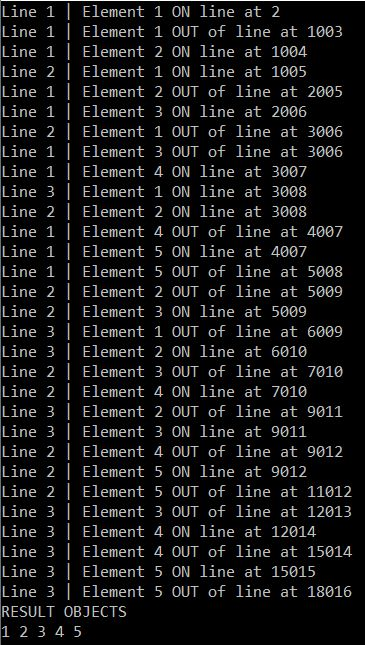
\includegraphics[scale=0.9]{result.jpg}}
		\caption{Результат работы программы}
	\end{figure}

	\subsection*{Вывод}
	\addcontentsline{toc}{subsection}{Вывод}
	По результаты работы программы можно сделать вывод, что действия, а именно начало обработки элементов и конец, выполняются параллельно. Конечный результат показывает, что последовательность элементов сохраняется.
	\clearpage
	
	\clearpage
	\section*{Заключение}
	\addcontentsline{toc}{section}{Заключение}
	В ходе выполнения лабораторной работы были изучены возможности параллельных вычислений и применены на примере конвейерной системы. Была разработан и описан конвейер с параллельно работающими линиями. Были даны ответствующие схемы. 
	
	Цель работы достигнута, все поставленные задачи выполнены.
	
	
	\newpage	
	\section*{Литература}
	\addcontentsline{toc}{section}{Литература}
		
	\begin{enumerate}
		\label{CPlusPlus}
		\item[1)] Бьерн Страуструп. Язык программирования С++. -URL:\par 
		\href{https://codernet.ru/books/c_plus/bern_straustrup_yazyk_programmirovaniya_c_specialnoe_izdanie/}
		{https://codernet.ru/books/c\_plus/bern\_straustrup\_yazyk\_programmirovaniya\_
			c\_specialnoe\_izdanie/}\par(дата обращения:
		01.10.2020). Текст: электронный.
		
		\label{Cute}
		\item[2)] Qt. -URL:\par
		\href{https://www.qt.io/}{https://www.qt.io/} (дата обращения: 01.10.2020). Текст: электронный.
		
		\label{CLOCK}
		\item[3)] Функция $clock$. -URL:\par
		\href{https://docs.microsoft.com/ru-ru/cpp/c-runtime-library/reference/clock?view=vs-2019}{https://docs.microsoft.com/ru-ru/cpp/c-runtime-library/reference/clock?view=vs-2019} (дата обращения:
		01.10.2020). Текст: электронный.
		
		\label{Conveyer}
		\item[4)] Конвейерное производство. -URL:\par \href{https://kartaslov.ru/карта-знаний/Конвейерное+производство}{https://kartaslov.ru/карта-знаний/Конвейерное+производство}\newline (дата обращения: 23.11.2020). Текст: электронный.
		
		
		%Дж. Макконнелл. Основы современных алгоритмов.\newline 2-е дополненное издание
		%\newline Москва: Техносфера, 2004. - 368с. ISBN 5-94836-005-9\newline
		%с. 130 - 133
		
		\label{ParInfo}
		\item[5)] Параллельные вычисления -URL:\par
		\href{https://ru.bmstu.wiki/}{https://ru.bmstu.wiki/} (дата обращения:
		13.11.2020). Текст: электронный.
		
	\end{enumerate}
\end{document}